\section{CFile\-Event\-Reactor  Class Reference}
\label{classCFileEvent_1_1CFileEventReactor}\index{CFileEvent::CFileEventReactor@{CFile\-Event::CFile\-Event\-Reactor}}
Inheritance diagram for CFile\-Event\-Reactor::\begin{figure}[H]
\begin{center}
\leavevmode
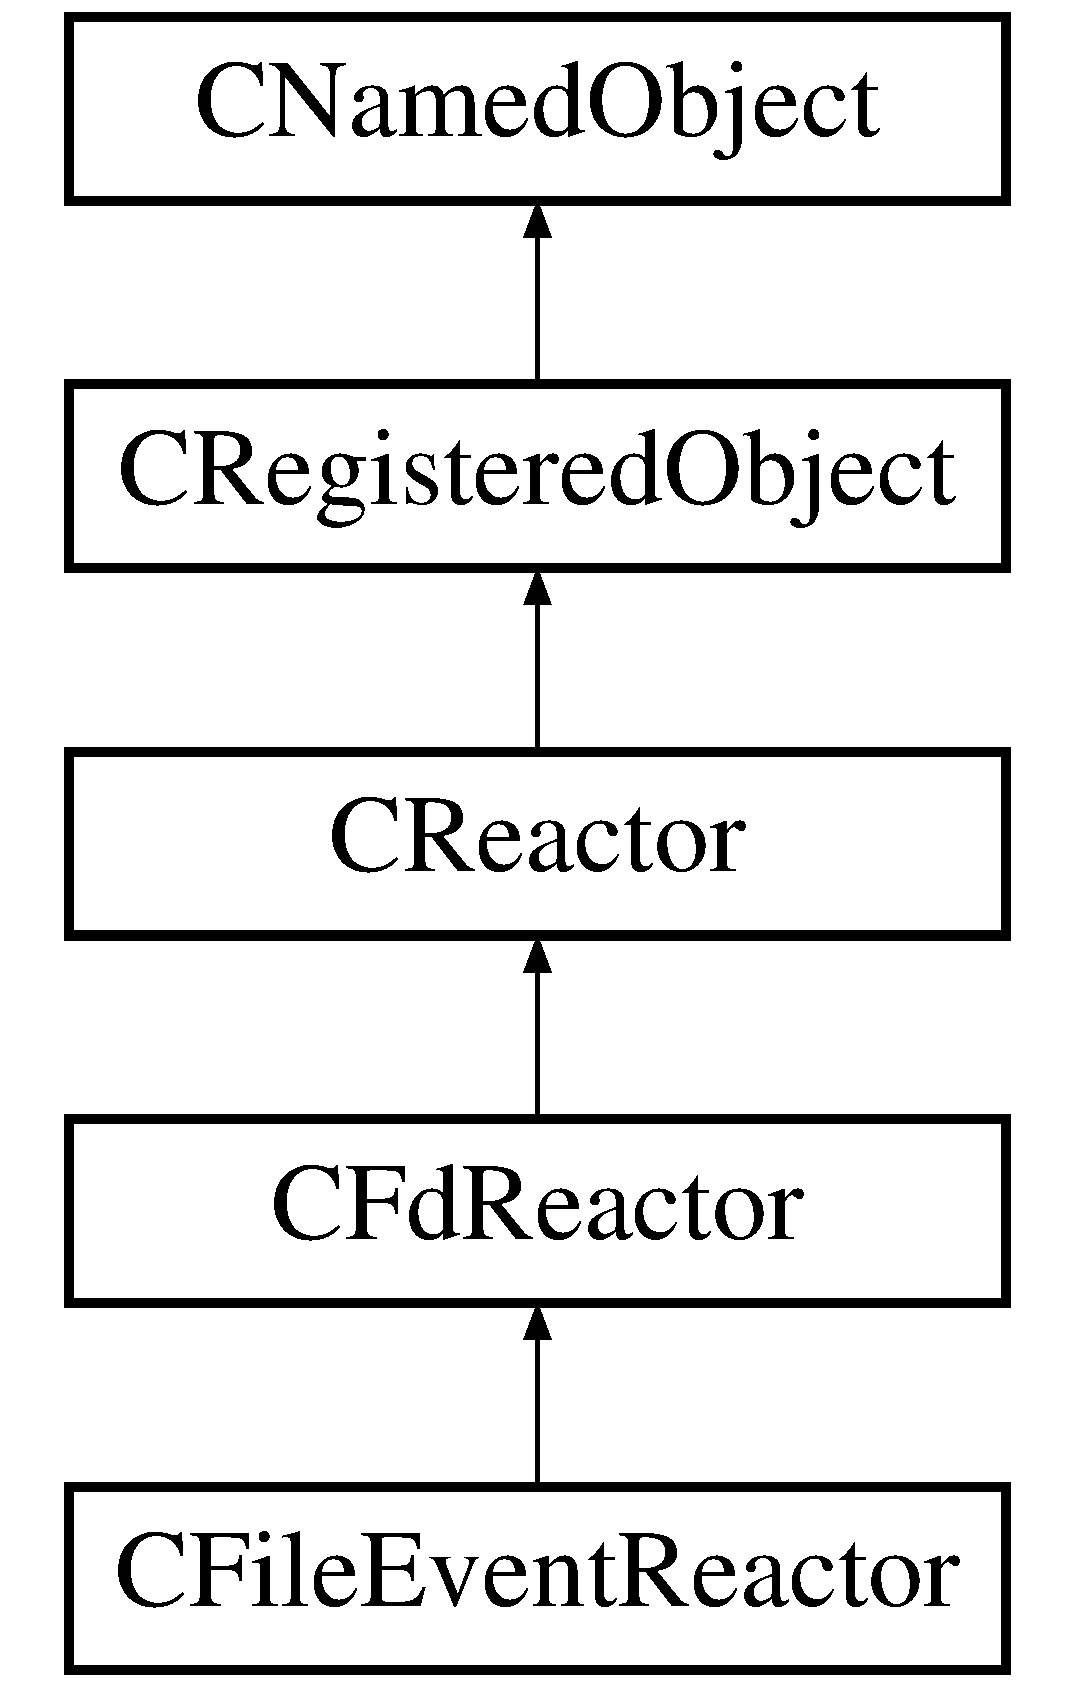
\includegraphics[height=5cm]{classCFileEvent_1_1CFileEventReactor}
\end{center}
\end{figure}
\subsection*{Public Methods}
\begin{CompactItemize}
\item 
{\bf CFile\-Event\-Reactor} (const string \&r\-Name, {\bf CFile\-Event} \&r\-Owner)
\item 
{\bf $\sim$CFile\-Event\-Reactor} ()
\item 
virtual void {\bf On\-Readable} ({\bf CFd\-Monitor} \&r\-Monitor, int fd)
\item 
virtual void {\bf On\-Writable} ({\bf CFd\-Monitor} \&r\-Monitor, int fd)
\item 
virtual void {\bf On\-Exception} ({\bf CFd\-Monitor} \&r\-Monitor, int fd)
\item 
virtual void {\bf On\-Timeout} ({\bf CEvent\-Monitor} \&r\-Monitor)
\end{CompactItemize}
\subsection*{Private Attributes}
\begin{CompactItemize}
\item 
{\bf CFile\-Event} \& {\bf m\_\-r\-Owner}
\begin{CompactList}\small\item\em Owner of us.\item\end{CompactList}\end{CompactItemize}


\subsection{Detailed Description}
This is an internal class which is automatically used as the  Reactor for File events. About the only thing it does is call back to the file event. 



Definition at line 342 of file CFile\-Event.h.

\subsection{Constructor \& Destructor Documentation}
\index{CFileEvent::CFileEventReactor@{CFile\-Event::CFile\-Event\-Reactor}!CFileEventReactor@{CFileEventReactor}}
\index{CFileEventReactor@{CFileEventReactor}!CFileEvent::CFileEventReactor@{CFile\-Event::CFile\-Event\-Reactor}}
\subsubsection{\setlength{\rightskip}{0pt plus 5cm}CFile\-Event\-Reactor::CFile\-Event\-Reactor (const string \& {\em r\-Name}, {\bf CFile\-Event} \& {\em r\-Owner})}\label{classCFileEvent_1_1CFileEventReactor_a0}


Constructor for {\bf CFile\-Event\-Reactor} {\rm (p.\,\pageref{classCFileEvent_1_1CFileEventReactor})}: Constructs the reactor by \begin{CompactItemize}
\item 
Calling the base class constructor ({\bf CReactor}() {\rm (p.\,\pageref{classCReactor_a0})}).\item 
Initializing m\_\-r\-Owner to the event which is instantiating us.\item 
Calling {\bf Append\-Class\-Info}() {\rm (p.\,\pageref{classCNamedObject_b2})} so that our place in the class hierarchy is well defined.\end{CompactItemize}
\begin{Desc}
\item[Parameters: ]\par
\begin{description}
\item[{\em 
r\-Name}]- Reference to the name given to this reactor. \item[{\em 
r\-Owner}]- Reference to the owning event. \end{description}
\end{Desc}


Definition at line 324 of file CFile\-Event.cpp.

References CNamed\-Object::Append\-Class\-Info().\index{CFileEvent::CFileEventReactor@{CFile\-Event::CFile\-Event\-Reactor}!~CFileEventReactor@{$\sim$CFileEventReactor}}
\index{~CFileEventReactor@{$\sim$CFileEventReactor}!CFileEvent::CFileEventReactor@{CFile\-Event::CFile\-Event\-Reactor}}
\subsubsection{\setlength{\rightskip}{0pt plus 5cm}CFile\-Event\-Reactor::$\sim$CFile\-Event\-Reactor ()\hspace{0.3cm}{\tt  [inline]}}\label{classCFileEvent_1_1CFileEventReactor_a1}




Definition at line 347 of file CFile\-Event.h.

\subsection{Member Function Documentation}
\index{CFileEvent::CFileEventReactor@{CFile\-Event::CFile\-Event\-Reactor}!OnException@{OnException}}
\index{OnException@{OnException}!CFileEvent::CFileEventReactor@{CFile\-Event::CFile\-Event\-Reactor}}
\subsubsection{\setlength{\rightskip}{0pt plus 5cm}void CFile\-Event\-Reactor::On\-Exception ({\bf CFd\-Monitor} \& {\em r\-Monitor}, int {\em fd})\hspace{0.3cm}{\tt  [virtual]}}\label{classCFileEvent_1_1CFileEventReactor_a4}


Called when an exceptional condition is encountered on a file. We create an iostream and bounce the call back to m\_\-r\-Owner's On\-Exception. This  creates the look and feel of a monolithic Event class. 

Reimplemented from {\bf CFd\-Reactor} {\rm (p.\,\pageref{classCFdReactor_a8})}.

Definition at line 371 of file CFile\-Event.cpp.

References CFile\-Event\-Reactor::m\_\-r\-Owner, and CFile\-Event::On\-Exception().\index{CFileEvent::CFileEventReactor@{CFile\-Event::CFile\-Event\-Reactor}!OnReadable@{OnReadable}}
\index{OnReadable@{OnReadable}!CFileEvent::CFileEventReactor@{CFile\-Event::CFile\-Event\-Reactor}}
\subsubsection{\setlength{\rightskip}{0pt plus 5cm}void CFile\-Event\-Reactor::On\-Readable ({\bf CFd\-Monitor} \& {\em r\-Monitor}, int {\em fd})\hspace{0.3cm}{\tt  [virtual]}}\label{classCFileEvent_1_1CFileEventReactor_a2}


Called whenever the file becomes readable. We create an istream for the file, and call back to m\_\-r\-Owner's On\-Readable member. This all makes the Event seem like a monolithic unit to the user.... They just subclass it, open a file in an appropriate way and poof.\begin{Desc}
\item[arm r\-Monitor - Refers to the monitor on the file (unused).]\par
 \end{Desc}
\begin{Desc}
\item[Parameters: ]\par
\begin{description}
\item[{\em 
fd}]- File descriptor open on the file. \end{description}
\end{Desc}


Reimplemented from {\bf CFd\-Reactor} {\rm (p.\,\pageref{classCFdReactor_a6})}.

Definition at line 342 of file CFile\-Event.cpp.

References CFile\-Event\-Reactor::m\_\-r\-Owner, and CFile\-Event::On\-Readable().\index{CFileEvent::CFileEventReactor@{CFile\-Event::CFile\-Event\-Reactor}!OnTimeout@{OnTimeout}}
\index{OnTimeout@{OnTimeout}!CFileEvent::CFileEventReactor@{CFile\-Event::CFile\-Event\-Reactor}}
\subsubsection{\setlength{\rightskip}{0pt plus 5cm}void CFile\-Event\-Reactor::On\-Timeout ({\bf CEvent\-Monitor} \& {\em r\-Monitor})\hspace{0.3cm}{\tt  [virtual]}}\label{classCFileEvent_1_1CFileEventReactor_a5}


Called when a wait on the file event times out. \begin{Desc}
\item[Parameters: ]\par
\begin{description}
\item[{\em 
r\-Monitor}]-referens to the event monitor. \end{description}
\end{Desc}


Reimplemented from {\bf CReactor} {\rm (p.\,\pageref{classCReactor_a8})}.

Definition at line 383 of file CFile\-Event.cpp.

References CFile\-Event::get\-Fd(), CFile\-Event\-Reactor::m\_\-r\-Owner, and CFile\-Event::On\-Timeout().\index{CFileEvent::CFileEventReactor@{CFile\-Event::CFile\-Event\-Reactor}!OnWritable@{OnWritable}}
\index{OnWritable@{OnWritable}!CFileEvent::CFileEventReactor@{CFile\-Event::CFile\-Event\-Reactor}}
\subsubsection{\setlength{\rightskip}{0pt plus 5cm}void CFile\-Event\-Reactor::On\-Writable ({\bf CFd\-Monitor} \& {\em r\-Monitor}, int {\em fd})\hspace{0.3cm}{\tt  [virtual]}}\label{classCFileEvent_1_1CFileEventReactor_a3}


Called when a file descriptor becomes writable. We just create a stream and bounce the call back to the {\bf CFile\-Event} {\rm (p.\,\pageref{classCFileEvent})}'s On\-Writable member. This presents a monolithic look and feel to the end user of this library.\begin{Desc}
\item[Parameters: ]\par
\begin{description}
\item[{\em 
r\-Monitor}]- The file monitor which declared the event.(unused) \item[{\em 
fd}]- The file id which is now writable  (constructs the ostream) \end{description}
\end{Desc}


Reimplemented from {\bf CFd\-Reactor} {\rm (p.\,\pageref{classCFdReactor_a7})}.

Definition at line 360 of file CFile\-Event.cpp.

References CFile\-Event\-Reactor::m\_\-r\-Owner, and CFile\-Event::On\-Writable().

\subsection{Member Data Documentation}
\index{CFileEvent::CFileEventReactor@{CFile\-Event::CFile\-Event\-Reactor}!m_rOwner@{m\_\-rOwner}}
\index{m_rOwner@{m\_\-rOwner}!CFileEvent::CFileEventReactor@{CFile\-Event::CFile\-Event\-Reactor}}
\subsubsection{\setlength{\rightskip}{0pt plus 5cm}{\bf CFile\-Event}\& CFile\-Event\-Reactor::m\_\-r\-Owner\hspace{0.3cm}{\tt  [private]}}\label{classCFileEvent_1_1CFileEventReactor_o0}


Owner of us.



Definition at line 344 of file CFile\-Event.h.

Referenced by CFile\-Event\-Reactor::On\-Exception(), CFile\-Event\-Reactor::On\-Readable(), CFile\-Event\-Reactor::On\-Timeout(), and CFile\-Event\-Reactor::On\-Writable().

The documentation for this class was generated from the following files:\begin{CompactItemize}
\item 
{\bf CFile\-Event.cpp}\item 
{\bf CFile\-Event.h}\end{CompactItemize}
